\begin{itemize}

    
    \item \textbf{uint8(x)} prints the byte that is located at the decimal position x, counted through a zero based indexing. The first byte from the the starting is at 0, second one is at 1 and so on.

     \item \textbf{uint32(x)} prints the word that is located at the start of decimal position x, counted through a zero based indexing. The word is located in order $x+3 \rightarrow x+2 \rightarrow x+1 \rightarrow x$ The word from the the starting is at order $3 \rightarrow 2 \rightarrow 1 \rightarrow 0$, second one is at $4 \rightarrow 3 \rightarrow 2 \rightarrow 1$ and so on.

     \item \textbf{filesize} prints the size of the file in bytes. The libxselinux.so file is of 24512 bytes.

     
\end{itemize}

\begin{figure}[H]

    \centering
    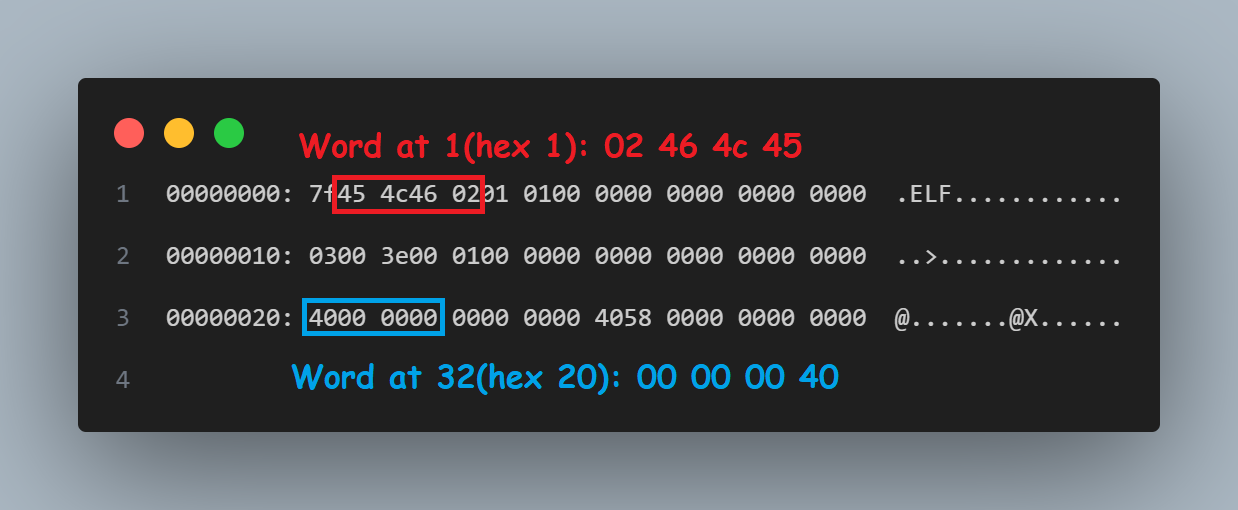
\includegraphics[width=\textwidth]{hex_file.png}
    \caption{Detecting position from hex file}
    \label{fig:file_hex}
    
\end{figure}

\section{Conclusion}

YARA rules are syntactically flexible and the architecture is also modular with a robust framework. With its extensive community support, YARA continues to evolve as a vital asset in the arsenal of cybersecurity professionals, enabling proactive defense measures against emerging threats and facilitating collaborative efforts in the fight against cybercrime.
